\section{Histoire}
\subsection{SCCS \& RCS}
\begin{frame}{SCCS \& RCS}
  \begin{columns}[T]

    \begin{column}{.5\textwidth}
      GNU SCCS (Source Code Control System), 1972
      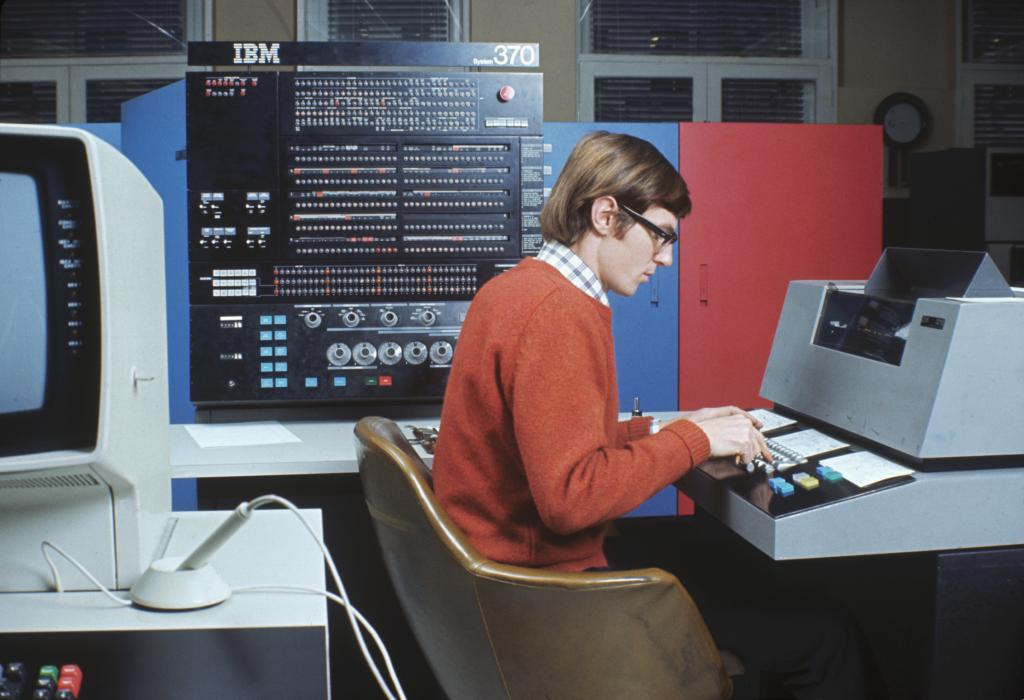
\includegraphics[width=\textwidth]{./ibm-system-370.png}
    \end{column}

    \begin{column}{.5\textwidth}
      GNU RCS (Revision Control System), 1982
      
\includegraphics[width=\textwidth]{./rcs-model.png}
    \end{column}

  \end{columns}
\end{frame}

\subsection{CVS \& SVN}
\begin{frame}{CVS \& SVN}
  \begin{columns}[T]

    \begin{column}{.5\textwidth}
      CVS (Concurrent Versions System), 1990
      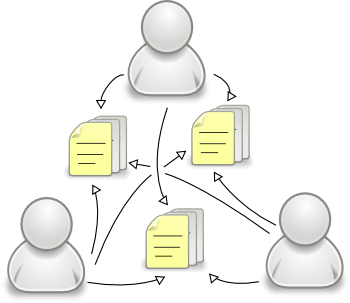
\includegraphics[width=\textwidth]{./cvs-model.png}
    \end{column}

    \begin{column}{.5\textwidth}
      SVN (Subversion), 2000
      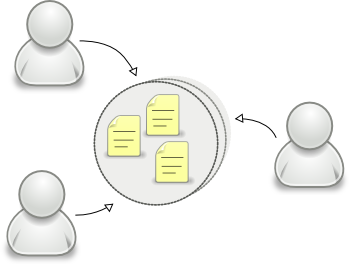
\includegraphics[width=\textwidth]{./svn-model.png}
    \end{column}

  \end{columns}
\end{frame}

\subsection{Git, Mercurial \& Bazaar}
\begin{frame}{Git, Mercurial \& Bazaar}
  \begin{columns}[T]

    \begin{column}{.5\textwidth}
      Git, 2005

      Mercurial, 2005

      GNU Bazaar, 2005
    \end{column}

    \begin{column}{.5\textwidth}
      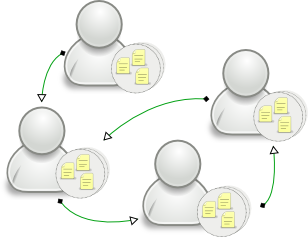
\includegraphics[width=\textwidth]{./hg-model.png}
    \end{column}

  \end{columns}
\end{frame}
